\pgfdeclarelayer{background}
\pgfdeclarelayer{foreground}
\pgfdeclarelayer{m-f}
\pgfdeclarelayer{main}

\pgfsetlayers{background,foreground}

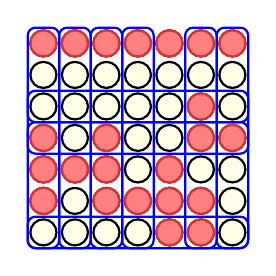
\begin{tikzpicture}
\tikzset
{
    vnodeStyle/.style = {circle, radius=1.8mm, thick,fill= yellow!10, text = black,draw = black,font = \scriptsize}
}

\clip  (-2mm,-2mm) rectangle (26mm, 26mm); 
\def\n     {6}

\begin{pgfonlayer}{background}
%\draw[gray,step=2mm] (-2mm,-2mm) grid (26mm, 26mm);
\foreach \rr in {0,1,...,\n}
 \foreach \cc in {0,1,...,\n}{
  \node[vnodeStyle] (p\rr\cc) at (\rr*4mm,\cc*4mm) {};
 }
\end{pgfonlayer}

\begin{pgfonlayer}{foreground}
\node[minimum width=10cm] (txt) at (12mm,-8mm) {};
\only<1>{ \node[minimum width=10cm] at (txt) {Product Code};
}

\uncover<2>{
 \node[minimum width=10cm] at (txt) {Received block};
}

\uncover<2-3>{
 \foreach \rr/\cc in {1/0,2/0,2/1,0/5,1/4,0/4,6/3,2/4,6/4,3/2,1/3,4/5,3/6,2/2,6/6,6/1}{
  \node[vnodeStyle,thick,fill=red!50,draw=red!80!black!80] (it1\rr\cc)
  at (\cc*4mm,\rr*4mm) {};
 }
}

\uncover<3-4>{
 \node[minimum width=10cm] at (txt) {Row decoding};
}

\uncover<3-3>{
 \node [rectangle,rounded corners=1mm,minimum width=\n*4mm+4mm,minimum height=4mm,draw=blue,thick] (circ2) at (3*4mm,4*4mm) {};
 \node [rectangle,rounded corners=1mm,minimum width=\n*4mm+4mm,minimum height=4mm,draw=blue,thick] (circ2) at (3*4mm,3*4mm) {};
 \node [rectangle,rounded corners=1mm,minimum width=\n*4mm+4mm,minimum height=4mm,draw=blue,thick] (circ2) at (3*4mm,0*4mm) {};
}

\uncover<4-6>{
 \foreach \rr/\cc in {1/0,2/0,2/1,1/4,6/3,2/4,6/4,1/3,2/2,6/6,6/1}{
  \node[vnodeStyle,thick,fill=red!50,draw=red!80!black!80] (it1\rr\cc)
  at (\cc*4mm,\rr*4mm) {};
 }
}

\uncover<5-6>{
 \node[minimum width=10cm] at (txt) {Column decoding};
}

\uncover<6-6>{
 \node [rectangle,rounded corners=1mm,minimum width=4mm,minimum height=\n*4mm+4mm,draw=blue,thick] (circ1) at (0*4mm,3*4mm) {};
 \node [rectangle,rounded corners=1mm,minimum width=4mm,minimum height=\n*4mm+4mm,draw=blue,thick] (circ1) at (1*4mm,3*4mm) {};
 \node [rectangle,rounded corners=1mm,minimum width=4mm,minimum height=\n*4mm+4mm,draw=blue,thick] (circ1) at (2*4mm,3*4mm) {};
 \node [rectangle,rounded corners=1mm,minimum width=4mm,minimum height=\n*4mm+4mm,draw=blue,thick] (circ1) at (3*4mm,3*4mm) {};
 \node [rectangle,rounded corners=1mm,minimum width=4mm,minimum height=\n*4mm+4mm,draw=blue,thick] (circ1) at (5*4mm,3*4mm) {};
 \node [rectangle,rounded corners=1mm,minimum width=4mm,minimum height=\n*4mm+4mm,draw=blue,thick] (circ1) at (6*4mm,3*4mm) {};
}

\uncover<7-7>{
 \foreach \rr/\cc in {1/4,2/4,6/4}{
  \node[vnodeStyle,thick,fill=red!50,draw=red!80!black!80] (it1\rr\cc)
  at (\cc*4mm,\rr*4mm) {};
 }
}

\uncover<8-8>{
 \node[minimum width=10cm] at (txt) {Decoding successful};
}


\uncover<9-9>{
 \node[minimum width=10cm] at (txt) {Or trapped in a \textcolor{red}{stopping set}};
 \foreach \rr/\cc in {1/0,3/0,6/0,1/2,3/2,6/2,1/5,3/5,6/5}{
  \node[vnodeStyle,thick,fill=red!50,draw=red!80!black!80] (it1\rr\cc)
  at (\cc*4mm,\rr*4mm) {};
 }
}
\end{pgfonlayer}
\end{tikzpicture}